\section{Sensitivity Analysis}

An important aspect of any fuel cycle transition scenario
is the accrual of fissile materials for new reactor deployment.
The collaborative strategy makes a transition possible 
from the perspective of material availability,
but the aggressive transition demands a significant increase in reprocessing capacity.

We explored the impact of two key variables, the lifetime of French \glspl{LWR} and the
breeding ratio of \gls{ASTRID} reactors. The range over which we varied these parameters (table \ref{tab:sen_par})
sought to capture the full span of their uncertainty.

Note that \gls{ASTRID} breeding ratios are arbitrarily increased
by direct adjustment of their output fuel compositions. We did not 
take into account the other reactor parameters (e.g. core size, initial
fuel composition, fuel residence time, etc.)
that would be neccessary to achieve a higher breeding ratio. More detailed analyses
of the reactor physics and their effect on this transition scenario 
should be pursued in future work.


\begin{table}[h]
    \centering
    \caption{Both \gls{LWR} lifetime and \gls{ASTRID} breeding ratio impact 
    transitional reprocessing demand.}
    \begin{tabularx}{\textwidth}{lrr}
        \hline
        \textbf{Parameter} & \textbf{Default} & \textbf{Values} \\
        \hline
        Breeding Ratio of \glspl{ASTRID} & 1.08 & 1.11, 1.15, 1.18 \\ 
        Lifetime of French \glspl{LWR} [years] & 60  & 65, 70, 80 \\
        \hline
    \end{tabularx}
    \label{tab:sen_par}
\end{table}

\subsection{Breeding Ratio}


Increase in the breeding ratio of \gls{ASTRID} reactors
decreases the total reprocessing demand, since less
\gls{UNF} must be reprocessed to extract the same amount of
plutonium. Additionally,
\glspl{ASTRID} become independent more quickly due to
higher breeding of plutonium.

Figure \ref{fig:br_fuel} shows the relationship between breeding ratio and fuel loading in \glspl{ASTRID}.
The \glspl{ASTRID} produce 
more plutonium, reducing the plutonium demand from 
reprocessed \gls{UOX}. However, since \gls{LWR} \gls{UNF} is not
the limiting factor for this transition scenario,
increasing the breeding ratio does not play a significant
role in the transition scenario, especially considering the technical difficulty
in achieving a high breeding ratio.

\begin{figure}[!ht]
	\centering
	\subfloat{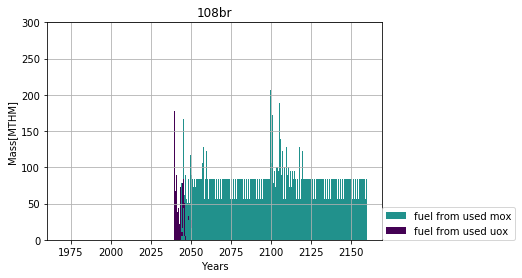
\includegraphics[width=.45\textwidth]{./images/sensitivity/108br.png}}\quad
	\subfloat{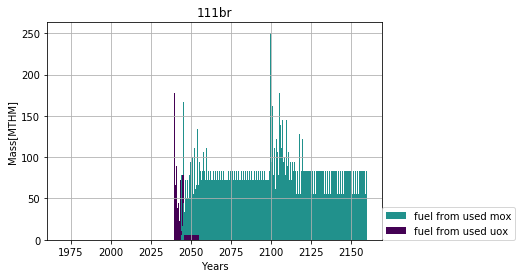
\includegraphics[width=.45\textwidth]{./images/sensitivity/111br.png}}\\
	\subfloat{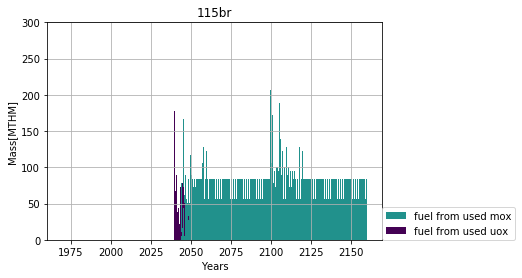
\includegraphics[width=.45\textwidth]{./images/sensitivity/115br.png}}\quad
	\subfloat{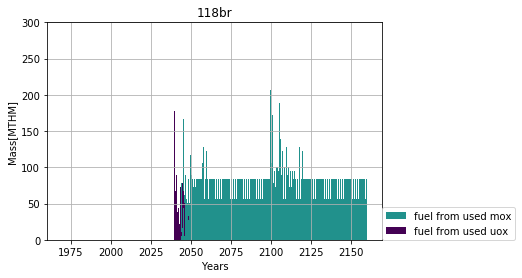
\includegraphics[width=.45\textwidth]{./images/sensitivity/118br.png}}
	\caption{\gls{ASTRID} fuel loading patters are altered by changes in \gls{ASTRID} 
		breeding ratio. Less \gls{ASTRID} fuel comes from reprocessed \gls{LWR} \gls{UNF}
		because \glspl{ASTRID} generate more plutonium.}
	\label{fig:br_fuel}
\end{figure}

The sensitivity analysis also shows, as demonstrated in figure \ref{fig:br_uox} that 
increasing the breeding ratio decreases the mass of \gls{LWR} \gls{UNF} 
required for the transition.

\begin{figure}[htbp!]
    \begin{center}
        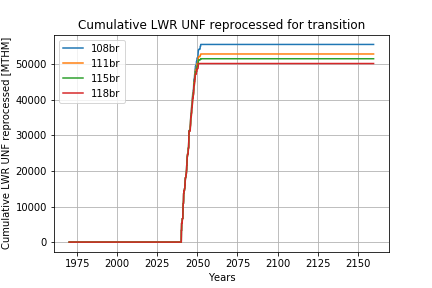
\includegraphics[scale=0.6]{./images/sensitivity/br_uox_unf_cum.png}
    \end{center}
    \caption{Sensitivity analysis demonstrates that increasing the breeding 
    ratio decreases the required \gls{UOX} \gls{UNF}. }
    \label{fig:br_uox}
\end{figure}

The differential impacts of varying the breeding ratios are
shown in table \ref{tab:br_diff}. The differences were calculated
using the following equation:

\[ \epsilon = \frac{(x - x_{base})}{x_{base}} * 100 \]

\begin{table}[h]
	\centering
        \caption{Breeding ratio impact on reprocessing requirements.}
	\begin{tabular}{lrrrr}
		\hline
                & \multicolumn{4}{c}{\% Difference} \\
		\textbf{Breeding Ratio $\longrightarrow$}& \textbf{1.08}& \textbf{1.11} & \textbf{1.15} & \textbf{1.18} \\
		\hline
		Total reprocessing demand & 0.0 & -5.3 & -7.8 & -10.3 \\ 
		\gls{LWR} \gls{UNF} reprocessed & 0.0  & -4.8 & -7.2 & -9.6 \\
		\hline
	\end{tabular}
	\label{tab:br_diff}
\end{table}


\subsection{Lifetime Extension of French \glspl{LWR}}\label{sec:life}
Extending the lifetime of French \glspl{LWR} lowers the average
monthly \gls{UOX} reprocessing demand, since the \gls{ASTRID} deployment becomes 
delayed (shown in figure \ref{fig:pow_diff}). The plutonium demand is delayed,
 allowing the reprocessing plant more time to prepare plutonium for \gls{ASTRID} reactors.

\begin{figure}[htbp!]
    \begin{center}
        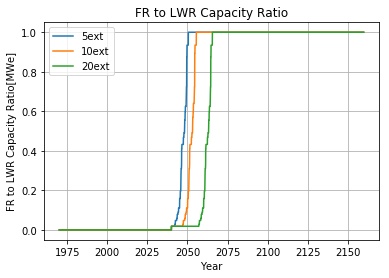
\includegraphics[scale=0.7]{./images/sensitivity/pow_ratio.png}
    \end{center}
    \caption{The ratio of \glspl{ASTRID} to \glspl{LWR} in France demarcates 
    the transition period.}
    \label{fig:pow_diff}
\end{figure}


Figure \ref{fig:ext_fuel} shows the change in \gls{ASTRID} fuel loading with
\gls{LWR} lifetime extension. The \gls{ASTRID} fuel loaded with plutonium
from \gls{LWR} \gls{UNF} conveys the corresponding \gls{LWR} \gls{UNF} reprocessing demand.
The change in \gls{ASTRID} deployment alters \gls{ASTRID} fuel loading patterns.
However, increasing the \gls{LWR} lifetimes
does not increase the \gls{LWR} \gls{UNF} demand significantly (less than 1\%
for the 20-year extension case),
because \glspl{ASTRID} become self-sustaining at similar times after the first
\gls{ASTRID} deployment.

\begin{figure}[!ht]
	\centering
	\subfloat{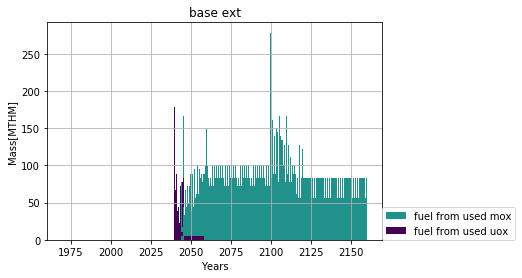
\includegraphics[width=.45\textwidth]{./images/sensitivity/base.png}}\quad
	\subfloat{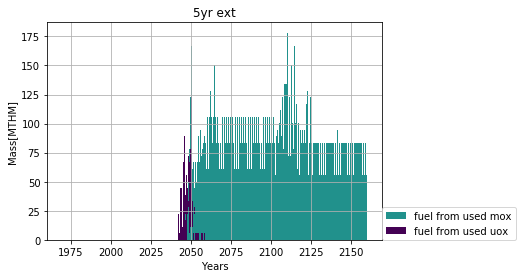
\includegraphics[width=.45\textwidth]{./images/sensitivity/5yr.png}}\\
	\subfloat{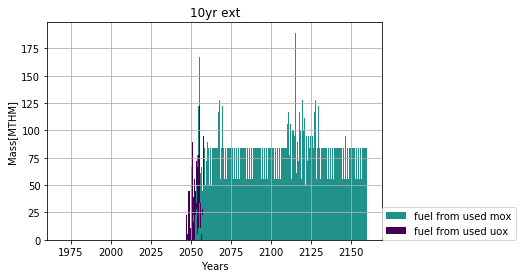
\includegraphics[width=.45\textwidth]{./images/sensitivity/10yr.png}}\quad
	\subfloat{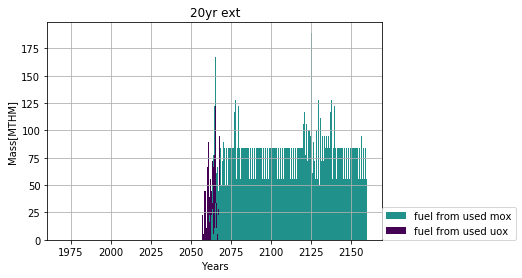
\includegraphics[width=.45\textwidth]{./images/sensitivity/20yr.png}}
	\caption{\gls{ASTRID} fuel loading patterns are altered by changes in \gls{ASTRID} deployment
			 caused by the lifetime extension of \glspl{LWR}.}
	\label{fig:ext_fuel}
\end{figure}

The quantitative effects of
\gls{LWR} lifetime extensions are shown in table \ref{tab:ext_met}.
The differences were calculated using the same equation used for the
breeding ratio study. 
Since \gls{LWR} lifetime extensions shorten the span of \gls{ASTRID} operations, less \gls{ASTRID} fuel is needed when \gls{LWR} lifetimes are extended.
Therefore, it is not fair to compare the mass of total \gls{UNF} reprocessed,
since less plutonium is extracted from \gls{UNF}. Instead, we compared the
average reprocessing values and the total amount of \gls{LWR} \gls{UNF} reprocessed.
There is not a significant difference (less than $1\%$ for the 20-year extension case)
in the amount of \gls{LWR}
\gls{UNF} reprocessed. The delay in \gls{ASTRID} deployment
spreads out the \gls{LWR} \gls{UNF} reprocessing demand,
thereby dramatically reducing ($39\%$ for the 20-year extension case)
the average monthly \gls{LWR} \gls{UNF} reprocessing demand.

\begin{table}[h]
	\centering
	\caption{\gls{LWR} lifetime extension impact on reprocessing requirements.}
	\begin{tabular}{lrrrr}
		\hline
		& \multicolumn{4}{c}{\% Difference} \\
		\textbf{\gls{LWR} lifetime extension $\longrightarrow$}& \textbf{0 years}& \textbf{5 years} & \textbf{10 years} & \textbf{20 years} \\
		\hline
		Total \gls{ASTRID} fuel produced & 0.0 & -3.9 & -8.0 & -16.3 \\
		\gls{LWR} \gls{UNF} reprocessed & 0.0  & -0.7 & -0.7 & -0.7 \\
		Average \gls{LWR} \gls{UNF} reprocessed & 0.0 & -16.0 & -25.7 & -39.8 \\
		Average \gls{UNF} reprocessed & 0.0 & -2.3 & -4.2 & -8.3 \\
		\hline
	\end{tabular}
	\label{tab:ext_met}
\end{table}
